\documentclass[10pt]{article}
\usepackage{fullpage}
\usepackage{amsmath}
\usepackage{amssymb}
\usepackage{amsfonts}
\usepackage{graphicx}
\usepackage{caption}
\usepackage{subcaption}

\DeclareMathOperator*{\argmin}{arg\,min}

\begin{document}

\section{System Design and Implementation}
% Section Overview
% Before we designed our system, we first implemented VQ and covq. We did this so we could expand on our code, but also so we could implement the independent decoders for comparing our system. We did implementation is C and Python, we also did some plotting in MATLAB. Mention that detailed design description is covered in design summary.

In the course of this project, we began by implementing a C program to perform simple Vector Quantization, and adapted it to an implementation of Channel-Optimized Vector Quantization by modifying the optimality conditions as was outlined in the Description section. We then wrote a C implementation of the I$\rightarrow$J system without a channel. To interface with images, we wrote a Python wrapper program. We also used GNU Octave, MathWorks MATLAB, and Python to produce data and create plots.\\

In the subsequent sections we will detail the design challenges that were faced along the way and how they were addressed.

\subsection{Conditions of Optimality}
% Nearest neighbour condition depends on other encoder -> Need to apply NN condition seperately. We chose to rotate between the three conditions of optimality in turn NN_X->NN_Y->CC.

Expanding for the optimality expressions given in [Description], we get that the optimal reconstruction of $X$, given fixed encoders and received codebook indices $k,l$ is given by

\begin{align}
    x_{(k,l)}&=
    \frac{
        \sum_{i=1}^{N_X}\sum_{j=1}^{N_Y}
            E[X|X\in R_i, Y\in S_j]P(k,l|i,j)
    }{
        \sum_{i=1}^{N_X}\sum_{j=1}^{N_Y}
            P(X\in R_i, Y\in S_j)P(k,l|i,j)
    }\\
    &=
    \frac{
        \sum_{i=1}^{N_X}\sum_{j=1}^{N_Y}
            P(k,l|i,j)\int_{x\in R_i}x
                \frac{
                    f_X(x)
                }{
                    P(X\in R_i, Y\in S_j)
                }dx
    }{
        \sum_{i=1}^{N_X}\sum_{j=1}^{N_Y}
            P(X\in R_i, Y\in S_j)P(k,l|i,j)
    }
\end{align}

Let $\mathcal T$ be a finite training set of ordered pairs drawn from the joint distribution for X and Y. Letting $M_{ij}$ be the number of training vectors in $R_i\times S_j$ we can thus approximate the integral and probabilities as follows:

\begin{align}
    x_{(k,l)}&=
    \frac{
        \sum_{i=1}^{N_X}\sum_{j=1}^{N_Y}
            P(k,l|i,j)\sum_{x\in R_i}x
                \frac{
                    1
                }{
                    M_{ij}
                }
    }{
        \sum_{i=1}^{N_X}\sum_{j=1}^{N_Y}
            P(X\in R_i, Y\in S_j)P(k,l|i,j)
    }
\end{align}

By symmetry, the optimal reconstruction for $Y$ is given by

\begin{align}
    y_{(k,l)}&=
    \frac{
        \sum_{i=1}^{N_X}\sum_{j=1}^{N_Y}
            P(k,l|i,j)\sum_{y\in S_j}y
                \frac{
                    1
                }{
                    M_{ij}
                }
    }{
        \sum_{i=1}^{N_X}\sum_{j=1}^{N_Y}
            P(X\in R_i, Y\in S_j)P(k,l|i,j)
    }
\end{align}

Similarly, we write out the nearest neighbour conditions; the idea is the same as in COVQ. The optimal encoding partitions for $X$ given fixed partitions in $Y$, and fixed decoding points $\{(x_{(k,l)},y_{(k,l)})\}$ are given by:

\begin{align}
    R_i &=
        \{x | d(x, i) \le d(x, h), \forall h\in \{1,...,N_X\}\}
\end{align}
\\
and symmetrically, the optimal encoding partitions for $Y$ given fixed partitions in $X$, and fixed decoding points $\{(x_{(k,l)},y_{(k,l)})\}$ are given by::

\begin{align}
    S_j &=
        \{y | d(y, j) \le d(y, h), \forall h\in \{1,...,N_Y\}\}
\end{align}
\\
where $d(x,i)$ is given by

\begin{align}
    d(x,i)=&E[Y^2 | X = x] +\\
    &\sum_{j=1}^{N_Y} \sum_{k=1}^{N_X} \sum_{l=1}^{N_Y} ( {(x-x_{(k,l)})}^2 -
    2y_{(k,l)}E[Y|X=x,Y\in S_j] + y_{(k,l)}^2 )P(Y\in S_j|X=x)
    P(k,l|i,j)\nonumber
\end{align}
\\
and $d(y, j)$ is given by

\begin{align}
        d(y,j)=&E[X^2 | Y = y] +\\
    &\sum_{i=1}^{N_X} \sum_{k=1}^{N_X} \sum_{l=1}^{N_Y} ( {(y-y_{(k,l)})}^2 -
    2x_{(k,l)}E[X|Y=y,X\in R_i] + x_{(k,l)}^2 )P(X\in R_i|Y=y)
    P(k,l|i,j)\nonumber
\end{align}

Here, we note how the nearest neighbour condition for $X$ depends on the $Y$ encoding regions $\{S_j\}$, and vice versa. We therefore adapt the Lloyd iteration into three stages. This poses a design issue with respect to (a) order of iteration and (b) initialization of codebook. The former we will address at the end of this section, the latter in the next section.\\

Focusing on $d(x,i)$, since $d(y, j)$ is analogous, we write out the expectations:

\begin{align}
    d(x,i)=&\int_{-\infty}^\infty y^2 f_{Y|X}(y|X=x)dy +\\
    &\sum_{j=1}^{N_Y} \sum_{k=1}^{N_X} \sum_{l=1}^{N_Y} ( {(x-x_{(k,l)})}^2 -
    2y_{(k,l)}\int_{-\infty}^\infty y^2 \frac{f_{Y|X}(y|X=x)}{P(Y\in S_j)}dy
     + y_{(k,l)}^2 )\int_{S_j} y f_{Y|X}(y|X=x)dy\cdot
    P(k,l|i,j)\nonumber
\end{align}

The part of this expression that poses a new problem is $f_{Y|X}(y|X=x)$. In order to approximate this with a finite training set, we can first quantize the training values with two one-dimensional uniform quantizers. This is formalized below.\\

Define
$q_X(x):\mathbb{R} \rightarrow \{x_1,\ldots,x_{L_X}\}$
and
$q_Y(y):\mathbb{R} \rightarrow \{y_1,\ldots,y_{L_Y}\}$
to be the $L_X$- and $L_Y$-level uniform quantizers for the sources $X$ and $Y$ respectively, where the $x_i-x_{i-1}$ is constant for all $i\in \{2,\ldots,L_X\}$, and $y_i-y_{i-1}$ constant for all $i\in \{2,\ldots,L_Y\}$

\begin{align}
    q_X(x) = x_i \in \{x_1,\ldots,x_{L_X}\} \iff x \in  \left[\frac{x_{i-1}+x_{i}}{2},\frac{x_i+x_{i+1}}{2}\right)\\
    q_Y(y) = y_i \in \{y_1,\ldots,y_{L_Y}\} \iff y \in  \left[\frac{y_{i-1}+y_{i}}{2},\frac{y_i+y_{i+1}}{2}\right)
\end{align}
\\
with the convention that $x_{0}=y_{0}=-\infty$, and $x_{L_X+1}=y_{L_Y+1}=+\infty$.\\

For simplicity of design, we attach this uniform quantizer to the beginning of our system. That is, we essentially transform the sources to have state spaces of size $L_X, L_Y$ before performing the I$\rightarrow$J quantization. (Modified block diagram)\\

We can now explicity rewrite our approximated conditions in computable terms via a uniformly quantized training set. First, we introduce some terms to simplify notation. Let $m(x_g, y_h)$ be the number of training pairs that quantize to the pair $(x_g,y_h)$:\\

\begin{align}
    m(x_g, y_h)&=|\{(x,y) \in \mathcal{T} : q_X(x) = x_g, q_Y(y) = y_h\}|\\
    \forall g&\in \{1,\ldots,L_X\}, \forall h\in \{1,\ldots,L_Y\}\nonumber
\end{align}

Let $I_X(x_g)\in\{1,\ldots,N_X\}$, $I_Y(y_h)$ be the index of `closest' $X$ codevector, $I_Y(y_h)\in\{1,\ldots,N_Y\}$ be the index of `closest' $Y$ codevector:

\begin{align}
    \label{eq:I_X}
    I_X(x_g)=\argmin_{i \in \{1,\dots,N_X\}}d_X(x_g,i)\\
    \label{eq:I_Y}
    I_Y(y_h)=\argmin_{j \in \{1,\dots,N_Y\}}d_Y(y_h,j)
\end{align}
\\
Notice that these are simply the nearest neighbour conditions for the uniformly quantized training set.\\

Let $M(x_g), M(y_h)$ be the number of training pairs that uniformly quantize to pairs of the form $(x_g, *)$, $(*, y_h)$ respectively:

\begin{align}
    M(x_g) &= {\sum_{h=1}^{L_Y}m(x_g,y_h)}\\
    M(y_h) &= {\sum_{g=1}^{L_X}m(x_g,y_h)}
\end{align}
\\
let $M_j(x_g)$ be the number of training pairs that uniformly quantize to pairs of the form $(x_g, y_h)$ with $y_h$ in the encoding region $S_j$, and $M_i(y_h)$ be the number of training pairs that uniformly quantize to pairs of the form $(x_g, y_h)$ with $x_g$ in the encoding region $R_i$:

\begin{align}
    M_j(x_g) &= \sum_{y_h:I_Y(y_h)=j}m(x_g,y_h) \\
    M_i(y_h) &= \sum_{x_g:I_X(x_g)=i}m(x_g,y_h)
\end{align}
\\
let $S_j(x_g), S_i(y_h)$ be given by:

\begin{align}
    S_j(x_g) &= \sum_{y_h:I_Y(y_h)=j}y_h\cdot m(x_g,y_h) \\
    S_i(y_h) &= \sum_{x_g:I_X(x_g)=i}x_g\cdot m(x_g,y_h)\\
\end{align}
\\
and $T(x_g), T(y_h)$ be given by:

\begin{align}
    T(x_g) &= \sum_{y_h=1}^{L_Y}y_h^2\cdot m(x_g,y_h)\\
    T(y_h) &= \sum_{x_g=1}^{L_X}x_g^2\cdot m(x_g,y_h)
\end{align}

We now rewrite $d_X, d_Y$ in the above terms. For shorthand, let $q_X(x)=x_g\in \{x_1,\ldots,x_{L_X}\}$ and $q_Y(y)=y_h\in \{y_1,\ldots,y_{L_Y}\}$

\begin{align}
    \label{eq:NN_X}
    d_X(x,i) =
            \frac{1}{M(x_g)} \bigg(T(x_g) + 
            \sum_{j=1}^{N_Y} \sum_{k=1}^{N_X} \sum_{l=1}^{N_Y}
            \Big(\big({(x-x_{(k,l)})}^2 +
            y_{(k,l)}^2\big)M_j(x_g) -2y_{(k,l)}S_j(x_g)\Big)P(k,l|i,j)\bigg)\\
    \label{eq:NN_Y}
    d_Y(y,j) =
            \frac{1}{M(y_h)} \bigg(T(y_h) + 
            \sum_{i=1}^{N_X} \sum_{k=1}^{N_X} \sum_{l=1}^{N_Y}
            \Big(\big({(y-y_{(k,l)})}^2 +
            x_{(k,l)}^2\big)M_i(y_h) -2x_{(k,l)}S_j(y_h)\Big)P(k,l|i,j)\bigg)
\end{align}
\\
\eqref{eq:NN_X} and \eqref{eq:NN_Y} are now easily computable for given pair $(x, i)$ or $(y, j)$, so the two nearest neighbour optimization steps reduce to performing a search over codebook indices $i$, $j$ respectively, for the solution to equations \eqref{eq:I_X}, \eqref{eq:I_Y} respectively.\\

We also note that, besides aiding notation, the terms $M_j(x_g),S_j(x_g),T(x_g)$, and their counterparts $M_i(y_h),S_i(y_h),T(y_h)$ can be computed initially, independent of $x_g, y_h$ respectively, reducing the computational complexity of the nearest neighbour lookup.\\

We now write out the centroid condition in a similar manner. We reiterate that the encoding partitions $\{R_i\}_{i=1}^{N_X}, \{S_j\}_{j=1}^{N_Y}$ are held constant in the application of this condition.\\

Let $M_{(i,j)}$ be the number of training vectors that belong to $R_i\times S_j$:

\begin{align}
    M_{(i,j)} &=
    \sum_{\substack{x_g:I_X(x_g)=i\\y_h:I_Y(y_h)=j}}m(x_g,y_h)
\end{align}
\\
and let $S_{(i,j)}^X$, $S_{(i,j)}^Y$ be given by:

\begin{align}
    S^X_{(i,j)} &=
    \sum_{\substack{x_g:I_X(x_g)=i\\y_h:I_Y(y_h)=j}}x_g\cdot m(x_g,y_h)\\
    S^Y_{(i,j)} &=
    \sum_{\substack{x':I_X(x')=i\\y':I_Y(y')=j}}y_h\cdot m(x_g,y_h)
\end{align}
\\
With the above notation, the reconstructions that minimize end-to-end distortion are:

\begin{align}
    \label{eq:C_X}
    x_{(k,l)} = 
        \frac{\sum_{i=1}^{N_X} \sum_{j=1}^{N_Y}
        S_{(i,j)}^X P(k,l|i,j)}
        {\sum_{i=1}^{N_X} \sum_{j=1}^{N_Y}
        M_{(i,j)} P(k,l|i,j)}\\
    \label{eq:C_Y}
    y_{(k,l)} = 
        \frac{\sum_{i=1}^{N_X} \sum_{j=1}^{N_Y}
        S_{(i,j)}^Y P(k,l|i,j)}
        {\sum_{i=1}^{N_X} \sum_{j=1}^{N_Y}
        M_{(i,j)} P(k,l|i,j)}
\end{align}
\\
Equations \eqref{eq:C_X}, \eqref{eq:C_Y} are now easily computable when our encoders are fixed.\\

Adding the uniform quantizer to the system presents new parameters. These are namely the choice of $\{x_1, y_1, x_{L_X}, y_{L_Y}, L_X, L_Y\}$. Together, these parameters control the granularity of quantization, and position of the quantizer. For our simulations, we chose to (a) center the quantizer about the sample mean of $\mathcal T$, (b) pick $\{x_1, y_1, x_{L_X}, y_{L_Y}\}$ such that all of $\mathcal T$ lies within the square defined by the four terms. With these decisions, the added complexity is simply how fine the quantizer ought to be.\\

For a given training set $\mathcal T$, we want fine enough quantization so to not distort the equations \eqref{eq:NN_X} and \eqref{eq:NN_Y}, but coarse enough so that the conditional probabilities are well-defined for most bins. It is clearly the case that with a larger training set $\mathcal T$, we can use finer quantizations while maintaining well-defined bins. For our purposes, we iterate through values of $L_X, L_Y$, choosing the result with lowest average distortion.\\

It is also important to note that the computational complexity depends primarily on the numbers $L_X, L_Y$, not the size of $\mathcal T$, as was the case in the I$\rightarrow$I system.\\

As was mentioned in this section, the fact that there are now three necessary conditions for optimality necessitates a decision in the order of their application in the quantizer training stage. We chose to give equal opportunities to each condition, beginning with one of the encoders. There are clearly other possible rotation schemes that might provide an advantage. These are not explored in this paper.\\

To summarize this section, we present the procedure which we dub the `Channel Optimized Stage' of our algorithm. Assuming we are given a codebook of size $N_X\cdot N_Y$, and the encoding mappings $I_X, I_Y$, we apply our modified Lloyd iteration to obtain a better set of encoding mappings and codebook.\\

\begin{enumerate}
    \item Store the previous distortion value, $D_{avg}$.
    \item Update the $X$ encoder; for each $x_g\in \{1,\ldots,L_X\}$, let
    \begin{align}
        I_X(x_g)=\argmin_{i\in\{1,\ldots,N_X\}}d_X(x_g,i)
    \end{align}
    \item Update the $Y$ encoder; for each $y_h\in \{1,\ldots,L_Y\}$, let
    \begin{align}
        I_Y(y_h)=\argmin_{i\in\{1,\ldots,N_Y\}}d_Y(y_h,j)
    \end{align}
    \item Update the codebook; for each $k\in\{1,\ldots,N_X\}$, $l\in\{1,\ldots,N_Y\}$ let
    \begin{align}
        x_{(k,l)} = 
            \frac{\sum_{i=1}^{N_X} \sum_{j=1}^{N_Y}
            S_{(i,j)}^X P(k,l|i,j)}
            {\sum_{i=1}^{N_X} \sum_{j=1}^{N_Y}
            M_{(i,j)} P(k,l|i,j)}\\
        y_{(k,l)} = 
            \frac{\sum_{i=1}^{N_X} \sum_{j=1}^{N_Y}
            S_{(i,j)}^Y P(k,l|i,j)}
            {\sum_{i=1}^{N_X} \sum_{j=1}^{N_Y}
            M_{(i,j)} P(k,l|i,j)}
    \end{align}
    \item Repeat until the average distortion changes less than a desired positive threshold, $\delta$; repeat if
    \begin{align}
        \frac
        {(D_{avg} - D^*_{avg})}
        {D_{avg}}
        > \delta
    \end{align}
    \\
    where $D_{avg}$ is the distortion of the previous iteration, and the new distortion $D^*_{avg}$ is given by
    \begin{align}
        D^*_{avg}=\frac{1}{M}\sum_{g=1}^{L_X}\sum_{h=1}^{L_Y}\left(M(x_g)\cdot d_X(x_g,I_X(x_g))+M(y_h)\cdot d_Y(y_h,I_Y(y_h))\right)
    \end{align}
\end{enumerate}

% Note this decision is somewhat arbitrary, the effects of other choices of order haven't been studied

% Design Problems: 
% Need conditional distributions for nearest neighbour condition -> Use Uniform Quantizer.
% Need to consider bin size. Bins too big and uniform quantizer adds distortion. Make bins too small and you can't approximate conditional distribution very well. Need a lot of training points for good approximation. 

% Another thing to note: complexity depends on total number of bins rather than number of training points.

% Present equations for conditions of optimality for training set/quantizer.

\subsection{Codebook Initialization}
% Describe problem
% Considered different methods of codebook initialization.

Since each nearest neighbour condition depends on the encoding regions of the other source and the codebook pairs $(x_{(k,l)},y_{(k,l)})$ of the decoder, and the joint centroid conditions depend on the encoding regions for both sources, it is necessary to appropriately find either (a) initial encoding regions $\{R_i\}, \{S_j\}$ for the encoders or (b) initial encoding regions for one of the sources and initial reconstruction points $\{(x_{(k,l)}, y_{(k,l)})\}$ for the decoder. We decided to do both, exploring a couple strategies.\\

% How did this work? we initialize reconstruction points, but then we still need to initialize one of the encoders..
% One method we tried was to initialize the reconstruction points $\{(x_{(k,l)}, y_{(k,l)})\}$ to the first $N_X\cdot N_Y$ training pairs in $\mathcal T$. This would ensure that the initial codebook would have the same distribution as $\mathcal T$ assuming that samples of $\mathcal T$ are independent and identically distributed. However, we found that 

To make finding initial encoding regions simpler, we took a heuristic approach to firstly initialize a codebook of the desired size, $\{(x_{(k,l)}, y_{(k,l)})\}$, $k=1\ldots N_X$, $l=1\ldots N_Y$, then apply suitable conditions to find initial encoding regions for \emph{both} sources, and finally begin the main iteration.\\

To find our initial codebook, our inspiration came from the Linde-Buzo-Gray (LBG) Splitting Algorithm. Recall that the LBG algorithm initializes the codebook to a single codevector, usually placed at the `center of mass' of the source distribution with respect to a distortion measure. We proceed in the same way, initially letting $N_X=N_Y=1$, with initial codebook pair $(x_{(1,1)},y_{(1,1)})$ given by: \\

\begin{align}
    x_{(1,1)} = \frac{1}{M}\sum_{g=1}^{L_X}\sum_{h=1}^{L_Y}x_g m(x_g, y_h)\\
    y_{(1,1)} = \frac{1}{M}\sum_{g=1}^{L_X}\sum_{h=1}^{L_Y}y_h m(x_g, y_h)
\end{align}
\\
which are respectively the expected values of the uniformly quantized training set for $X$ and $Y$. Trivially, our encoders are given by:\\

\begin{align}
    I_X(x) = 1\\
    I_Y(y) = 1
\end{align}

We then define the average distortion from this choice of codebook as the expected value of the sum of the squared error distortion between the quantized training vectors in $\mathcal T$ and the codebook:

\begin{align}
    D_{avg}^* = \frac{1}{M}\sum_{g=1}^{L_X}\sum_{h=1}^{L_Y}((x_g-x_{(1,1)})^2+(y_h-y_{(1,1)})^2)\cdot m(x_g,y_h)
\end{align}

We then split in the $X$ and apply a modified Lloyd iteration described as follows.\\

\begin{enumerate}
    
    \item \label{init_split} Split in $X$: let $N_X=2N_X$.
    \item \label{init_start} Remember previous distortion; let $D_{avg}=D^*_{avg}$
    \item Update the $X$ encoder; for each $g\in\{1,\ldots,L_X\}$ let
    \begin{align}
        I_X(x_g) = \argmin_{i \in \{1,\dots,N_X\}}d_X(x_g,i)
    \end{align}
    \\
    where $d_X(x_g,i)$ is given as in \eqref{eq:NN_X}, however with zero probability of channel error:
    \begin{align}
        \label{eq:no_channel_NN}
        d_X(x_g,i) =
            \frac{1}{M(x_g)} \bigg(T(x_g) + 
            \sum_{j=1}^{N_Y}
            \Big(\big({(x_g-x_{(i,j)})}^2 +
            y_{(i,j)}^2\big)M_j(x_g) -2y_{(i,j)}S_j(x_g)\Big)\bigg)
    \end{align}
    \item Update the $X$ codebook values; for each $k\in \{1,\ldots,N_X\}$, $l\in\{1,\ldots,N_Y\}$, let
    \begin{align}
        x_{(i,j)} = 
            \frac{\sum_{\substack{x_g:I_X(x_g)=i\\y_h:I_Y(y_h)=j}}x_g\cdot m(x_g,y_h)}
            {\sum_{\substack{x_g:I_X(x_g)=i\\y_h:I_Y(y_h)=j}}m(x_g,y_h)}
    \end{align}
    Notice that this is the expected value of the partition $(i,j)$.
    \item Update the $Y$ encoder; for each $h\in \{1,\ldots,L_Y\}$, let
    \begin{align}
        I_Y(y_h) = \argmin_{j\in\{1,\ldots,N_Y\}}d_Y(y_h,j)
    \end{align}
    where $d_Y(y_h,j)$ is defined in the same way as $d_X(x_g,i)$ in \eqref{eq:no_channel_NN}, i.e. we let the channel error probability of \eqref{eq:NN_Y} be zero.
    \item Update the $Y$ codebook values; for each $k\in \{1,\ldots,N_X\}$, $l\in\{1,\ldots,N_Y\}$, let
    \begin{align}
        y_{(i,j)} = 
            \frac{\sum_{\substack{x_g:I_X(x_g)=i\\y_h:I_Y(y_h)=j}}y_h\cdot m(x_g,y_h)}
            {\sum_{\substack{x_g:I_X(x_g)=i\\y_h:I_Y(y_h)=j}}m(x_g,y_h)}
    \end{align}
    \item Define the average distortion. let
    \begin{align}
        D_{avg}^* = \frac{1}{M}\sum_{h=1}^{L_Y}d_Y(y_h, I_Y(y_h))\left(\sum_{g=1}^{L_X}m(x_g,y_h)\right)
    \end{align}
    \item If
        $\frac
        {(D_{avg} - D^*_{avg})}
        {D_{avg}}
        > \delta$
        then return to step \ref{init_start},\\
        otherwise if $N_X$ is less than desired, go to next split (step \ref{init_split}),\\
        otherwise finish.
\end{enumerate}

After convergence of the iteration for our final value of $N_X$, we then apply the symmetric splitting algorithm in $Y$ until we reach our desired codebook size $N_Y$ in the $Y$. This yields an initial codebook optimized with respect to the dependence between $X$ and $Y$. It is worth noting that the properties of the channel do not enter this stage at all; this was a conscious choice that allows for the channel to not be defined for codebooks of size less than $N_X\cdot N_Y$.\\

The above routine we dub the `Initialization Stage', we follow this with the `Channel Optimization Stage' which was described in the previous section.

% Implementation:
% Tried Assigning codevectors to first N training points. Didn't work very well
% Tried splitting Algorithm. Advantage: can initialize encoders more easily. Should converge to a more optimal solution.

% Need to consider how to initialize encoders since you can't initialize one encoder using nearest neighbour conditions without having the other one already initialized.
% Splitting makes this simple

\subsection{Codeword Assignment}
% Need to map indices onto binary codewords. Present minimization problem. Problem is NP-complete.
% build this up from point-to-point case
% show minimization objective function of the codeword maps b_X, b_Y

Thus far, our algorithm optimizes the mappings $I_X, I_Y$ from source pairs onto codebook pairs, and the codebook $\{(x_{(k,l)}, y_{(k,l)})\}$ subject to the minimization of our distortion functions $d_X, d_Y$. Since this optimization does not ensure a globally optimal solution, it is possible for the iteration to converge to a sub-optimal configuration. Hence, it ``doesn't hurt'' to find other ways to optimize the system. We introduce the mappings $b_X, b_Y$ as the .\\

Define the channel index sets of $X$ and $Y$ respectively to be $\{1,\ldots,N_X\}, \{1,\ldots,N_Y\}$; for convenience, these are numbered in the same way as the encoding index sets. We require that there be an invertible mapping (i.e. a permutation) between encoding indices for each source and their respective channel index set. We call these mappings $b_X(i), b_Y(j)$ respectively. We also denote their inverses $b^{-1}_X(i'), b^{-1}_Y(j')$, where we use the convention that ``primed'' indices are channel indices.\\

The optimization problem alluded to above is that of minimizing the average end-to-end distortion by changing the mappings $b_X, b_Y$ for a fixed encoders, $I_X, I_Y$, and fixed codebook $\{(x_{(k,l)}, y_{(k,l)})\}$, $k=1,\ldots,N_X$, $l=1,\ldots,N_Y$.\\

Following the construction of \ref{} for the point-to-point case, we adapt the proof to our system. Expressing the objective function in terms of our index mappings and our quantizers gives:

\begin{align}
    D(I_X, I_Y, b_X, b_Y)&=
        E\left[(X-x_{(K,L)})^2+(Y-y_{(K,L)})^2; b_X, b_Y\right]\\
    % &= E\left[(X-x_{(K,L)})^2; b_X, b_Y\right]+E\left[(Y-y_{(K,L)})^2; b_X, b_Y\right]
    &= \sum_{i,j}P(I_X(X)=i,I_Y(Y)=j)E\left[(X-x_{(K,L)})^2+(Y-y_{(K,L)})^2|I_X(X)=i, I_Y(Y)=j; b_X, b_Y\right]\\
    &= \sum_{i,j}p(i,j)\sum_{k,l}p(b(k),b(l)|b(i),b(j))E\left[((X-x_{(k,l)})^2+(Y-y_{(k,l)})^2)) | I_X(X)=i, I_Y(Y)=j; b_X, b_Y\right]\\
    &= \sum_{i,j}p(i,j)\sum_{k,l}p(b_X^{-1}(k),b_Y^{-1}(l)|b_X(i),b_Y(j))
        \iint_{\substack{x: I_X(x)=i\\y: I_Y(y)=j}}
            (x-x_{(k,l)})^2+(y-y_{(k,l)})^2dxdy\\
    &=blah
    % &\qquad\qquad\qquad\qquad\qquad\qquad\qquad E\left[d(X,\B{\hat x}_{kl})+d(Y,\B{\hat y}_{kl})|X\in S^X_i, Y\in S^Y_j\right]\\
    % &= \sum_{i,j}p(i,j)\sum_{k,l}p(g_1^{-1}(\B{\hat x}_{kl}, \B{\hat y}_{kl}),g_2^{-1}(\B{\hat x}_{kl}, \B{\hat y}_{kl})|b_X(\B{\hat x}_i),b_Y(\B{\hat y}_j))\cdot {}\\
    % &\qquad\qquad\qquad\qquad\sum_{(\B{x}, \B{y})\in S_{ij}}p(\B{x},\B{y} | (\B{x}, \B{y})\in S_{ij})\cdot(d(\B{x},\B{\hat x}_{kl})+d(\B{y},\B{\hat y}_{kl}))
\end{align}

\begin{align}
    \label{eq:energy}
    D_C(b_X,b_Y)=
        \sum_{i,j}
            \sum_{k,l}
            P(b_X^{-1}(k), b_Y^{-1}(l) | b_X(i), b_Y(j))\cdot
            \left((x_{(i,j)}-x_{(k,l)})^2+(y_{(i,j)}-y_{(k,l)})^2\right)
\end{align}

%Implementation:
% Simulated annealing
% show 
The minimization of this function is an NP hard problem. We use the probabilistic method of Simulated Annealing to find a good approximation to the globally optimal solution.\\

Simulated Annealing works by iteratively choosing `neighbour states' at random from the `state space', and probabilistically deciding whether or not to transition to that state based on how long we've been searching and whether or not the new state is `lower energy' than the current state.\\

In our case, the functions $b_X,b_Y$ define the state space, and we define a `neighbour state' of a given $(b_X, b_Y)$ to be a pair $(b'_X, b'_Y)$ such that $b_X(i)\neq b'_X(i)$ for at most two values of $i$ and $b_Y(j)\neq b'_Y(j)$ for at most two values of $j$. The `energy' function that we are trying to minimize is \eqref{eq:energy}.\\

We now describe the algorithm in terms of our functions. We require a few parameters that together control the amount of time spent searching the state space. Define:

\begin{equation}
    \{T_i=10,T_f=0.00025,R=0.8,\phi_{max}=5,\psi_{max}=200\}
\end{equation}

In words, these are respectively: the initial `temperature', the final `temperature', the `cooling rate', the number of energy drops until we lower the temperature, the number rejected new states until we lower the temperature. These values are taken from \ref{}. We stop our search when our timing variable the `temperature' equals $T_f$.

\begin{enumerate}
    \item Initialize $b_X, b_Y$ to the identity maps:
    \begin{align}
        b_X(i) = i,  \quad\forall i\in \{1,\ldots,N_X\}\\
        b_Y(j) = j, \quad\forall j\in \{1,\ldots,N_Y\}
    \end{align}
    \item Initialize temperature $T$; let $T=T_i$.
    \item Initialize counters; let $\phi=0$, $\psi=0$
    \item Initialize `best' channel index maps; let
    \begin{align}
        b_{X_{best}}&=b_X\\
        b_{Y_{best}}&=b_Y
    \end{align}
    \item \label{anneal_loop}
    At random, choose $i_1, i_2\in \{1,\ldots,N_X\}$, choose $j_1,j_2\in \{1,\ldots,N_Y\}$. Define $b'_X,b'_Y$ as follows:
    \begin{align}
        b'_X(i) = 
            \begin{cases}
                b_X(i_1) &\mbox{if } i=i_2\\
                b_X(i_2) &\mbox{if } i=i_1\\
                b_X(i)  &\mbox{otherwise}
            \end{cases}\\
        b'_Y(i) = 
            \begin{cases}
                b_Y(j_1) &\mbox{if } j=j_2\\
                b_Y(j_2) &\mbox{if } j=j_1\\
                b_Y(j)  &\mbox{otherwise}
            \end{cases}
    \end{align}
    \begin{enumerate}
        \item If $D_C(b'_X,b'_Y)<D_C(b_X,b_Y)$, accept the change; let
            \begin{align}
                b_X&=b'_X\\
                b_Y&=b'_Y
            \end{align}
        \item If $D_C(b'_X,b'_Y)\ge D_C(b_X,b_Y)$, accept the change with probability $\exp(\frac{-(D_C(b'_X,b'_Y)- D_C(b_X,b_Y))}{T})$.
        \item Otherwise, keep the current state.
    \end{enumerate}
    \item If $D_C(b_X, b_Y) < D_C(b_{X_{best}}, b_{Y_{best}})$, store this `best' state; let
    \begin{align}
        b_{X_{best}}&=b_X\\
        b_{Y_{best}}&=b_Y
    \end{align}
    \item
    \begin{enumerate}
        \item If we accepted the change, increment $\phi$; let $\phi=\phi+1$
        \item Otherwise, increment $\psi$; let $\psi=\psi+1$
    \end{enumerate}
    \item
    \begin{enumerate}
        \item If $\psi=\psi_{max}$, reset $\psi$, lower temperature; let
        \begin{align}
            \psi &= 0\\
            T &= R\cdot T
        \end{align}
        \item Otherwise, if $\phi=\phi_{max}$, reset $\phi$, lower temperature; let
        \begin{align}
            \phi &= 0\\
            T &= R\cdot T
        \end{align}
        \item Otherwise, leave temperature unchanged.
    \end{enumerate}
    \item 
    \begin{enumerate}
        \item If $T > T_f$, go back to step \ref{anneal_loop}
        \item Otherwise, restore best state; let
        \begin{align}
            b_X&=b_{X_{best}}\\
            b_Y&=b_{Y_{best}}
        \end{align}
    \end{enumerate}

\end{enumerate}

\subsection{Image Coding}
% Presented problems with what to input to quantizer -> DCT blocks
% Bit allocation (we did not explore this for joint decoder case)

Since our system is suited for two correlated sources, we decided to apply it to the compression of two images that ought to (intuitively) share spatial correlation. The class of images we focused on was the class of stereoscopic images - that is, pairs of images of the same setting taken from two different angles. We explore the effect of transform coding on pairs of images from this class as input to our system.\\

Transform coding is often used in practice for efficient image coding \ref{}. The concept behind transform coding is to perform an \emph{orthogonal} linear transform on large blocks of the source scalars prior to scalar quantization, then inverse transformed on the decoding side. This is illustrated in (Figure??). The reason this is done is to pairwise \emph{de-correlate} the components of the input vector such that the components of the output vector of the transform are (close to) pairwise uncorrelated \ref{}.\\

Of the known computable orthogonal linear transforms, the Discrete Cosine Transform (DCT or DCT-II) has been found to be the most effective \ref{}, and it is widely used in image and video compression. A 2-D DCT is often used on blocks of 8$\times$8 pixels of the source image before lossy quantization, e.g. JPEG, JPEG-2000. We give the 2-D DCT for 8$\times$8 pixel blocks $\{x_{i,j}\}, i=0\ldots 7, j=0\ldots 7$ below:

\begin{equation}
    \left\{X_{i', j'}=\sum_{i=0}^7\sum_{j=0}^7
        x_{i,j}
            \cos\left[
                \frac{\pi}{8}\left(j+\frac{1}{2}\right)j'
            \right]
            \cos\left[
            \frac{\pi}{8}\left(i + \frac{1}{2}\right)i'
            \right]\right\}\quad i'=0\ldots 7, j'=0\ldots 7
\end{equation}

\begin{figure}
    
    \centering
    \begin{subfigure}{0.5\textwidth}
        \centering
        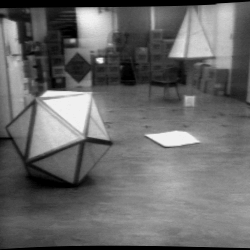
\includegraphics[width=0.6\linewidth]{img/cart_orig_left.png}
        \caption{left}
    \end{subfigure}% <- this percent sign is important 8)
    \begin{subfigure}{0.5\textwidth}
        \centering
        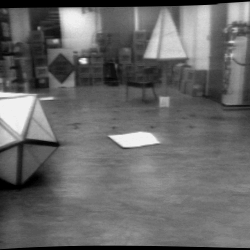
\includegraphics[width=0.6\linewidth]{img/cart_orig_right.png}
        \caption{right}
    \end{subfigure}
    \caption{An example of a stereo image.}
    \label{fig:cart_orig}
\end{figure}

The database of freely licenced stereo images we used was found at \ref{}. An example of the type of image we used is shown in figure \ref{fig:cart_orig}.\\

\begin{figure}
    \begin{subfigure}{0.5\textwidth}
        \begin{equation*}
            \left[
            \begin{matrix}
                7 & 7 & 5 & 4 & 0 & 0 & 0 & 0 \\
                7 & 5 & 4 & 0 & 0 & 0 & 0 & 0 \\
                6 & 5 & 0 & 0 & 0 & 0 & 0 & 0 \\
                5 & 0 & 0 & 0 & 0 & 0 & 0 & 0 \\
                5 & 0 & 0 & 0 & 0 & 0 & 0 & 0 \\
                4 & 0 & 0 & 0 & 0 & 0 & 0 & 0 \\
                0 & 0 & 0 & 0 & 0 & 0 & 0 & 0 \\
                0 & 0 & 0 & 0 & 0 & 0 & 0 & 0
            \end{matrix}
            \right]
        \end{equation*}
    \caption{left}
    \end{subfigure}%
    \begin{subfigure}{0.5\textwidth}
        \begin{equation*}
            \left[
            \begin{matrix}
                7 & 6 & 5 & 3 & 0 & 0 & 0 & 0 \\
                7 & 4 & 4 & 0 & 0 & 0 & 0 & 0 \\
                6 & 4 & 0 & 0 & 0 & 0 & 0 & 0 \\
                5 & 0 & 0 & 0 & 0 & 0 & 0 & 0 \\
                5 & 0 & 0 & 0 & 0 & 0 & 0 & 0 \\
                4 & 0 & 0 & 0 & 0 & 0 & 0 & 0 \\
                4 & 0 & 0 & 0 & 0 & 0 & 0 & 0 \\
                0 & 0 & 0 & 0 & 0 & 0 & 0 & 0
            \end{matrix}
            \right]
        \end{equation*}
    \caption{right}
    \end{subfigure}
    \caption{Greedy independent 64 bit allocation for the stereo images of figure \ref{fig:cart_orig} }
    \label{fig:cart_bit_alloc}
\end{figure}

An important question in transform coding is that of bit allocation. We wish to know how many bits, i.e. how many codevectors, to assign to each DCT coefficient to optimally recover the source. In the single source case, this problem was studied in \ref{julien}. A simple greedy algorithm optimally allocates bits to the DCT coefficients. The algorithm assumes that the $(0,0)$ coefficient (the DC coefficient) is Gaussian, while the other 63 coefficients are Laplacian \ref{julien}. An example of how this algorithm allocates bits to the images of figure \ref{fig:cart_orig} is given in figure \ref{fig:cart_bit_alloc}.\\

\begin{figure}
    \begin{equation*}
        \left[
        \begin{matrix}
        0.443 & -0.01  & -0.093 & -0.011 & -0.061 &   0.003 & -0.017 &  0.062 \\
        0.416 &  0.006 & -0.011 &  0.014 & -0.031 &  -0.039 &  0.003 & -0.045 \\
        0.498 & -0.061 & -0.01  &  0.074 & -0.034 &  -0.017 &  0.008 &  0.054 \\
        0.438 &  0.027 & -0.008 &  0.074 & -0.016 &   0.022 &  0.006 & -0.004 \\
        0.449 &  0.075 & -0.019 &  0.017 &  0.014 &   0.063 & -0.029 &  0.007 \\
        0.632 &  0.028 & -0.034 & -0.018 &  0.033 &  -0.037 &  0.032 &  0.061 \\
        0.765 &  0.177 & -0.032 & -0.063 & -0.033 &   0.076 & -0.001 &  0.089 \\
        0.679 &  0.148 &  0.028 &  0.04  &  0.046 &  -0.013 &  0.046 &  0.034
        \end{matrix}
        \right]
    \end{equation*}
    \caption{DCT coefficient correlation matrix of the stereo images in figure \ref{fig:cart_orig} }
\end{figure}

\begin{figure}
    \begin{equation*}
        \left[
        \begin{matrix}
        0.654 & 0.134 & 0.054 & 0.087 & 0.077 & 0.124 & 0.119 & 0.144 \\
        0.371 & 0.072 & 0.043 & 0.059 & 0.05  & 0.063 & 0.053 & 0.048 \\
        0.273 & 0.067 & 0.065 & 0.06  & 0.055 & 0.05  & 0.062 & 0.059 \\
        0.23  & 0.056 & 0.064 & 0.053 & 0.046 & 0.045 & 0.047 & 0.039 \\
        0.242 & 0.053 & 0.05  & 0.056 & 0.047 & 0.062 & 0.058 & 0.036 \\
        0.213 & 0.064 & 0.064 & 0.05  & 0.061 & 0.052 & 0.045 & 0.059 \\
        0.238 & 0.068 & 0.07  & 0.056 & 0.048 & 0.046 & 0.042 & 0.054 \\
        0.233 & 0.081 & 0.074 & 0.066 & 0.046 & 0.05  & 0.039 & 0.049
        \end{matrix}
        \right]
    \end{equation*}
    \caption{Average DCT coefficient correlation matrix of the dataset of 39 pairs of stereo images}
\end{figure}

The DCT computations and image manipulation was coded in Python using Pillow Imaging library and numpy.\\

The bit allocation problem for the two source case was not studied. We have thus omitted bit allocation from our simulations.

% Implementation:
% Python PILLOW library & numpy

\subsection{Design Summary}
% Summary initialization scheme in summary. We also have two stages : training stage (which is performed offline) and running stage which is used during simulation.
To recap, and to provide an overall picture, we will now give an overview of the system design. The following describes our process for images.\\

\begin{enumerate}
    \item Convert pixel data of stereo images to 64 scalar pair sets of 2-D DCT coefficients;
    \item Find good bit allocation using the optimal bit allocation greedy algorithm for independent sources;
    \item Perform `Initialization Stage' quantization with splitting;
    \item \label{channel_opt_stage}
    Perform `Channel-Optimization Stage' quantization until convergence;
    \item Perform simulated annealing to find approximately optimal channel codeword mappings $b_X, b_Y$;
    \item Return to step \ref{channel_opt_stage} until satisfactory distortion is achieved.
\end{enumerate}

% Summarize design and talk about complexity.
% [unif Q_X] -> [enc X] -> [b_X] \
%                                 --> [MAC]-- [Joint decode]
% [unif Q_Y] -> [enc Y] -> [b_Y] /



\end{document}
